%!TEX root = ../trabajo.tex
\capitulo{Marco Teórico}
El presente marco teórico sustentará la investigación para la realización del diseño de un algoritmo para la selección de proyectos de aplicaciones móviles a partir de criterios imprecisos. En este apartado se exponen los antecedentes y las bases teóricas del anteproyecto. Dichas bases teóricas consisten en una revisión bibliográfica e interpretación de fuentes primarias y secundarias relevantes al tópico de investigación propuesto.  Para la selección del material se toman en cuenta temas relacionados con términos incluidos en el título del trabajo de grado propuesto, tales como: selección de proyectos, atributos borrosos, y desarrollo de aplicaciones móviles. Además, asociados con estos tópicos y con el concepto de toma de decisiones, hay otros temas cuya explicación puede considerarse como parte de los basamentos teóricos: la selección de alternativas, conjuntos borrosos, medidas de comparación entre conjuntos borrosos, sistemas de información, y comparación de objetos con múltiples atributos borrosos.\\
\\
A continuación, se presentan los antecedentes relacionados con la investigación a desarrollar, así como las bases teóricas que la sustentan.

\seccion{Antecedentes de la Investigación}
Los antecedentes serán presentados cronológicamente por áreas temáticas asociadas, iniciando con el desarrollo de software para aplicaciones móviles, seguido por las investigaciones relacionadas al proceso de toma de decisiones.\\  
\\
\citet{wasserman2010software} presenta el trabajo ``Software engineering issues for mobile application development'' donde proporciona una visión general de importantes temas de investigación de ingeniería de software relacionados con el desarrollo de aplicaciones que se ejecutan en dispositivos móviles. Entre los temas más relevantes planteados por el autor se encuentran los procesos de desarrollo, herramientas, diseño de la interfaz de usuario, la portabilidad de las aplicaciones, calidad y seguridad de las mismas. Esta investigación ha sido referenciada por \citet{jiang2015software}, donde describen la situación actual respecto a los desafios y oportunidades que se presentan en el desarrollo de software para dispositivos moviles.  Dentro del análisis realizado por los autores se destacan aspectos que permiten obtener una mejor comprensión de las prácticas para el desarrollo de aplicaciones móviles, entre los cuales se encuentran los siguientes:
\begin{enumeracion}
\item La mayoría de las aplicaciones son relativamente pequeñas, con un promedio de varios miles de líneas de código fuente, con uno o dos desarrolladores responsables de la concepción, el diseño y la implementación de la aplicación.
\item Se presenta una marcada división entre las aplicaciones ``nativas'', las que se ejecutan en su totalidad en el dispositivo móvil, y las aplicaciones con manejo de servicios web.
\item Los desarrolladores suelen utilizar los aspectos recomendados para el desarrollo de ``mejores prácticas'', pero rara vez emplean un proceso de desarrollo formal.
\item Los desarrolladores hacen muy poco seguimiento organizado de sus esfuerzos de desarrollo.
\end{enumeracion}
\\
Dentro de este trabajo  se destaca la importancia de los criterios identificados por Wasserman y Jiang, debido a que estos serán fundamentales en la bitácora de análisis que se realizará para la selección de criterios en el desarrollo de esta investigación.\\
\\
Desde otra perspectiva, \citet{Narayan2014Mobile} plantea el desarrollo de aplicaciones móviles como un proceso complejo, debido a que las plataformas de los sistemas operativos móviles difieren en sus tecnologías ---lenguaje de programación, ejecución, enfoque---, además de la dificultad que presenta el aprender las diferentes tecnologías tanto para la comunidad de desarrolladores, como para empresas dedicadas a esta actividad, teniendo en cuenta la necesidad de ampliar y diversificar los nichos del mercado, lo que según el autor genera poca factibilidad en el uso de plataformas para desarrollos nativos, planteando así un reto en la creación de aplicaciones en función de distintos factores, como son el costo de desarrollo, tecnología de desarrollo a seleccionar, personal experto (``Full-Stack Developer''), curva de aprendizaje para los desarrolladores menos expertos, entre otros.\\
\\
A continuación se presentan algunos de los criterios tomados en cuenta en la investigación de Nayaran:
\\
\begin{viñetas}
\item Soporte de plataformas de sistemas operativos móviles.
\item Aprovechamiento de las capacidades del Dispositivo.
\item Curva de Aprendizaje.
\item Impacto en tiempo de desarrollo regular.
\item Rendimiento.
\item Empaquetamiento y distribución.
\item Costo de la plataforma, modelo de licencia y mantenimiento.
\\
\end{viñetas}
El autor en su investigación se encarga de hacer una comparación de las características a tomar en cuenta al seleccionar una tecnología o plataforma de desarrollo híbrida, como es el caso de Xamarin, Phone-gap y Appcelerator  siendo este contenido de gran aporte para la identificar criterios desde una nueva perspectiva en la evaluación de proyectos de aplicaciones móviles. Uno de los aportes importantes de este trabajo de grado será la incorporación de las dos visiones de desarrollo ---plataformas de desarrollo nativas e híbridas--- dando una visión más global de las características presentes en este mercado.\\
\\
Para realizar una comparación y posterior selección entre los distintos proyectos de aplicaciones móviles, no solo es necesaria la caracterización del problema, también es requerido el contar con formas de análisis y evaluación de dichos proyectos. \citet{bashon2013framework}, en su investigación titulada “A framework for comparing heterogeneous objects: on the similarity measurements for fuzzy, numerical and categorical attributes”, presentan un método de medición de similitud que combina enfoques clásicos (por ejemplo numérico, categórico) y  difusos, para  hacer la comparación de objetos que tengan diferentes tipos de datos.\\
\\
Los autores clasifican los atributos de los objetos de la siguiente manera:\\

\begin{viñetas}
\item \textit{Atributos con valores nítidos (o numéricos):} cada atributo tiene un dominio básico bien definido (llamado el universo de discurso) U ⊆ ℝ que es por lo general un conjunto acotado.
\item \textit{Atributos categóricos:} tienen valores de un conjunto discreto y fijo de términos lingüísticos. 
\item \textit{Atributos difusos:} cada atributo representa un conjunto de etiquetas lingüísticas que representan valores imprecisos y que pueden ser descritos fácilmente por un conjunto $F(U) = {A \vert A \subseteq U}$ de subconjuntos difusos definidos sobre la base de un dominio $U$. Cada sub-conjunto difuso $A \in F(U)$ es caracterizado por una función de  pertenencia: $\mu_{A} :U \rightarrow [0,1]$.
\\
\end{viñetas}
El objetivo de los autores es proporcionar un método para comparar los atributos clásicos (numéricos y categóricos) y  los atributos difusos, luego combinarlos con medidas de similitud. Esto con el fin de presentar un método unificado de combinación de medidas de similitud definido para comparar objetos con atributos numéricos, categóricos y difusos.\\
\\
Esta investigación presenta aportes de interés para este trabajo de grado, mostrando la importancia de tratar las colecciones de datos presentes en el mundo real y de naturaleza generalmente heterogénea (representadas por un conjunto de tipos de datos con atributos mixtos: numéricos, categóricos y difusos); mediante el uso de un marco de nuevas y unificadas medidas de similitud para comparar objetos heterogéneos descritos por atributos numéricos, categóricos y difusos.\\
\\
Estos factores de similitud presentados por Bashon, serán incorporarlos en este estudio (método de comparación y selección), con el fin de  comparar los objetos con atributos heterogéneos, que combinan enfoques clásicos y difusos en una medida de similitud unificada.\\
\\
\citet{Gupta2015fuzzyAhpTopsis}, presentan un análisis comparativo de la técnica para el orden de preferencia por Similitud con Solución Ideal (``Technique for Order of Preference by Similarity to Ideal Solution'', TOPSIS) y del proceso jerárquico analítico borroso (``Fuzzy Analytic Hierarchy Process'', Fuzzy AHP) en el contexto de la toma de decisiones para una selección de diseño. Esta comparación se hizo con base en factores ambientales, de calidad, costo y ergonomía. Para ilustrar el modelo propuesto, fueron considerados varios conceptos sobre bolsos de equipaje, y el determinar el más apropiado. Además, los autores realizaron un análisis de correlación para comparar el orden de jerarquización obtenido por los métodos TOPSIS y Fuzzy AHP. Los dos métodos son ejecutados separadamente, y las puntuaciones finales se convierten y califican en una escala de cero (0) a uno (1), para facilitar la comparación.\\
\\
Los dos enfoques sirven para el mismo propósito, pero mientras el método Fuzzy AHP mide el desempeño en una estructura jerárquica mediante el uso de matriz de comparación por pares, el método TOPSIS lo mide mediante el uso de la distancia a principios ideales positivos y negativos. Como resultado, se observa que el orden de prioridad resulta ser el mismo, pero la puntuación de los pesos relativos varía. Los requerimientos de entrada del método Fuzzy AHP son mayores que los del método TOPSIS, lo cual puede resultar más tedioso para el usuario. Por otra parte, el tiempo del programa para el método computacional del Fuzzy AHP es mayor que el del método TOPSIS, por lo que para aplicaciones complejas pudiera ser más conveniente el TOPSIS. Es difícil definir cuál de los métodos es el apropiado para la presente investigación pues dependiendo del grado de borrosidad, naturaleza subjetiva, complejidad e independencia de criterio y consistencia, puede variar la elección de implementar uno de los dos métodos. El procedimiento y resultados de esta investigación proveen de información aprovechable en cuanto a la forma de implementar un prototipo de sistema para probar la metodología que se desea diseñar, por ejemplo en cuanto al ambiente computacional a utilizar, y las medidas de comparación entre varias propuestas para mejorar la metodología.\\
\\
Siguiendo con el análisis de criterios, \citet{tom2015fuzzy} formulan la necesidad de evaluar menús de restaurantes mediante un modelo de toma de decisión difusa. El proceso de comparación y elección de opciones de menú más saludables se convierte en una tarea que consume tiempo y es difícil debido a las grandes cantidades de elementos que conforman el menú y la nutrición total disponible de cada comida (asociada a la suma nutricional de cada uno de los elementos del menú que forman parte de cada comida). 
Los autores plantearon este problema de selección como un problema de toma de decisión multicriterio, proponiendo un algoritmo para la toma de decisiones basado en los elementos presentes en cada plato, utilizando  criterios difusos priorizados elegidos por los clientes para la selección de comida en un menú. Este clasificador para menús de restaurante se puede aplicar a diferentes tipos de alimentación fuera del hogar  incluyendo comida de restaurantes de servicio completo, para llevar, y los servicios de comida rápida.
Esta investigación se tendrá en cuenta en el presente trabajo por su similitud en características respecto al algoritmo propuesto para calcular el índice de desempeño de las alternativas, ya que un menú incluye categorías y subcategorías, y cada elemento de menú tiene múltiples nutrientes críticos para ser evaluados, además los distintos consumidores pueden tener diferentes preferencias en función de sus condiciones de salud y otras preferencias.
\seccion{Bases Teóricas}
Se presenta a continuación una serie de conceptos asociados al desarrollo de un algoritmo basado en lógica difusa para la selección de proyectos móviles con atributos imprecisos.

\subseccion{Conjuntos difusos y lógica difusa}
De acuerdo con la teoría clásica de conjuntos, un elemento o pertenece a un conjunto, o se encuentra fuera del conjunto. No existe la situación intermedia. No existe un elemento con pertenencia parcial a un conjunto. Un ejemplo de esta situación es la estatura de una persona. De acuerdo con la lógica clásica se considera que una persona es alta a partir de determinada estatura, por ejemplo $1,80 m.$; lo que, según esa dicotomía puede llevar a calificar de baja a una persona de $1.79 m.$ En cambio, según la teoría de conjuntos borrosos, puede existir un elemento con una pertenencia parcial a un conjunto. Si un elemento es parcialmente miembro de un conjunto, también es parcialmente no miembro del mismo conjunto. Dado que la teoría de conjuntos difusos permite la pertenencia gradual de un elemento a un conjunto, puede considerarse como una generalización de la teoría clásica de conjuntos \cite[]{negnevitsky2005artificial, zadeh2008there}.\\
\\
Los conjuntos difusos fueron propuestos originalmente para hacer frente a los problemas de incertidumbre subjetiva. La incertidumbre subjetiva como resultado del uso de variables lingüísticas para representar un problema o  evento. Se debe tener en cuenta que una variable lingüística es una variable que se expresa por medio de palabras o frases verbales en un lenguaje natural o artificial. Por ejemplo, las variables lingüísticas con números difusos triangulares pueden tomar valores como ``muy bueno'', ``buen'', ``regular'', ``malo'', y ``muy malo'', como se muestra en el \refgrafico{graficoVariables}, para indicar las funciones de pertenencia de los valores de expresión.
\begin{grafico}[titulo = Función de pertenencia de algunas variables lingüísticas, etiqueta=graficoVariables]
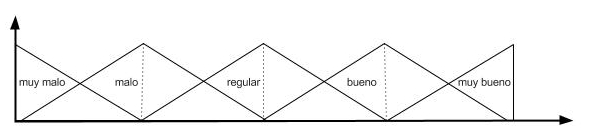
\includegraphics[width=15cm]{graficas/variables.jpg}
\end{grafico}
La adopción de variables lingüísticas recientemente se ha generalizado y se utiliza para evaluar las calificaciones lingüísticas dadas por los evaluadores. Por otra parte, las variables lingüísticas se emplean también como una forma de medir el logro del valor de rendimiento para cada criterio.\\
\\
El término de “conjunto difuso” (o conjunto borroso), aparece por primera vez en los años sesenta cuando el profesor Lotfi A. \citet{zadeh1965fuzzy}, de la Universidad de Berkeley en USA, publica un artículo titulado ``Fuzzy sets''. Luego de esta publicación, Zadeh ha iniciado líneas de investigación fundamentales sobre el análisis de sistemas complejos y los procesos de toma de decisiones, la lógica difusa y sus implicaciones en diversos dominios tales como el razonamiento aproximado, la gestión de la incertidumbre, los sistemas expertos, las redes neuronales, la información granular y su centralidad en el razonamiento humano, la computación con palabras.
Por ejemplo, se consulta un grupo de personas y se establecen las funciones de pertenencia para las temperaturas ``fría'', ``normal'' y ``caliente'' que se representan mediante conjuntos difusos; y se obtiene como resultado lo indicado en el \refgrafico{graficoTemperaturas}:

\begin{grafico}[titulo = Funciones de pertenencia para algunas temperaturas, etiqueta=graficoTemperaturas]
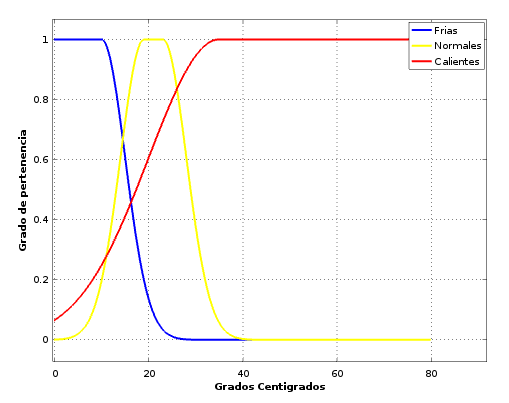
\includegraphics[width=12cm]{graficas/temparaturas.png}
\end{grafico}
Se observa que para el caso de temperatura ``normal'', en la región alrededor de 22º C se tiene un grado de pertenencia igual a 1, mientras que para valores menores o iguales a 10º C y mayores o iguales a 40º C, el grado de pertenencia es cero.\\
\\
Entre los tipos de funciones de pertenencia que más se usan en la especificación de números difusos están las de forma triangular, trapezoidal, gaussiana y de campana generalizada, las cuales pueden definirse de manera conveniente y concisa mediante fórmulas matemáticas parametrizadas \cite[]{jang1997neuro}. El \refcuadro{tablaModeloDM} muestra las fórmulas y parámetros de estas funciones.\\

\begin{cuadro}[titulo= Fórmulas y parámetros de funciones de pertenencia, etiqueta = tablaModeloDM]{|p{1.9cm}|c|c|}
\hline
\textbf{Tipo de Función} & \textbf{Fórmulas} & \textbf{Parámetros} \\
\hline
 & & \\
\textit{Triangular} & 
${ \mu  }_{ A }(x)=\left\{ \begin{matrix} 0\quad \quad \Leftrightarrow \quad (x\le a\quad \vee \quad x\ge c) \\ \cfrac { x-a }{ b-a } \quad \quad \Leftrightarrow \quad \quad \quad a\le x\le b \\ \cfrac { c-x }{ c-b } \quad \quad \Leftrightarrow \quad \quad \quad b\le x\le c\quad  \end{matrix} \right $
& $a, b, c$ \\
 & & \\
\textit{Trapezoidal} &
 ${ \mu  }_{ A }(x)=\left\{ \begin{matrix} 0\quad \quad \Leftrightarrow \quad (x\le a\quad \vee \quad x\ge d) \\ \cfrac { x-a }{ b-a } \quad \Leftrightarrow \quad \quad  a\le x\le b \\ 1\quad \quad \quad  \Leftrightarrow \quad \quad b\le x\le c \\ \cfrac { d-x }{ d-c } \quad \Leftrightarrow \quad  \quad c\le x\le d\quad  \end{matrix} \right $ 
 & $a, b, c, d$ \\
 & & \\
\textit{Gaussiana} 
& 
${ \mu  }_{ A }(x)={ e }^{ -{ 1 }/{ 2 }{ ((x-c)-\sigma ) }^{ 2 } }$
& $c, \sigma$\\ 
 & & \\
\textit{Campana generalizada}
& 
${ \mu  }_{ A }(x)=\cfrac { 1 }{ 1+{ \left| \cfrac { x-c }{ a }  \right|  }^{ 2b } }$
& $a, b, c$\\
 & & \\
 \hline
\end{cuadro}
\fuentecuadro{3}{ \citet[pp. 25-26]{jang2002neuro}}
\subseccion{Relaciones y operaciones básicas entre conjuntos difusos}

A continuación se describen dos relaciones y cuatro operaciones estandarizadas, con base en dos conjuntos difusos cualesquiera $A, B$ en el mismo universo $X$ \cite[pp. 21-23]{jang2002neuro}.

\subsubseccion{Igualdad}
 Se dice que $A$ es igual a $B$ si y sólo si para cada elemento $x \in X$, los números reales $\mu_{A}(x)$ y $\mu_{B}(x)$ son iguales. Se denota $A = B$.
\subsubseccion{Subconjunto}
Se dice que $A$ es un subconjunto de $B$ si y sólo si para cada elemento $x \in X$, el número real  $\mu_{A}(x)$  es menor que el número real  $\mu_{B}(x)$   , o ambos números reales son iguales. Se denota $A \subseteq B$.
\subsubseccion{Unión}
La unión estándar de $A$ y $B$ es el conjunto difuso $C$ en $X$, tal que su función de pertenencia $\mu_{C}:X \rightarrow [0, 1]$ está definida por $\mu_{C}(x)=\max {{\{\mu_{A}(x),\mu_{B}(x)\}}}$ para cada $x \in X$. Se denota $A \cup B$. \\
El \refgrafico{graficoUnion} muestra la unión estándar de dos conjuntos difusos con funciones de pertenencia triangulares.
\begin{grafico}[titulo = Union estandar en conjuntos difusos, etiqueta=graficoUnion]
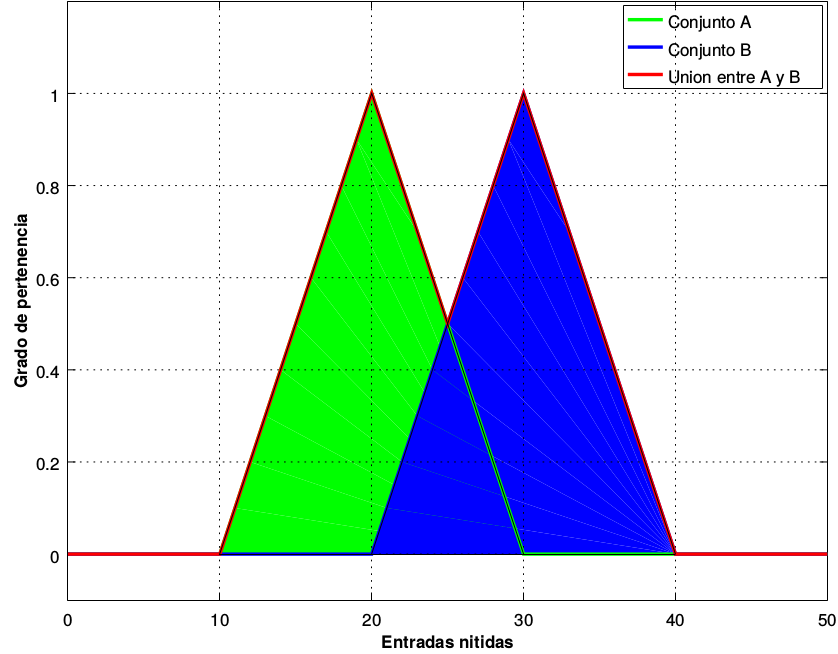
\includegraphics[width=8cm]{graficas/union.png}
\end{grafico}
\subsubseccion{Intersección}
La intersección estándar de $A$ y $B$ es el conjunto difuso $C$ en $X$, tal que su función de pertenencia $\mu_{C}(x):X \rightarrow [0, 1]$ está definida mediante la proposición $\mu_{C}= \min \{\mu_{A}(x), \mu_{B}(x) \}$ para cada $x \in X$. Se denota $A \cap B$.\\
El \refgrafico{graficoInterseccion} muestra la intersección estándar entre dos conjuntos difusos con funciones de pertenencia triangulares.
\begin{grafico}[titulo = Intersección estandar en conjuntos difusos, etiqueta = graficoInterseccion]
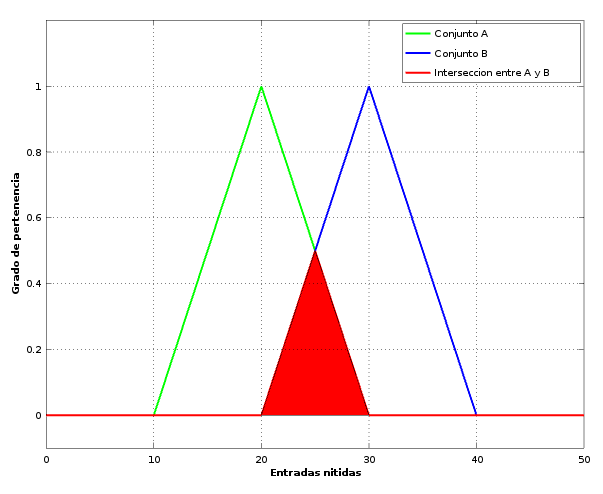
\includegraphics[width=8cm]{graficas/interseccion.png}
\end{grafico}
\subsubseccion{Complemento}
El complemento estándar de $A$ es el conjunto difuso $C$ en $X$, tal que su función de pertenencia $\mu_{C}(x):X \rightarrow [0, 1]$ está definida por $\mu_{C}(x)=1 -\mu_{A}(x)$ para cada $x \in X$. Se denota $\bar{A}$.\\
El \refgrafico{graficoComplemento} muestra el complemento estándar de un conjunto difuso con función de pertenencia triangular.
\begin{grafico}[titulo = Complemento estandar en conjuntos difusos, etiqueta = graficoComplemento]
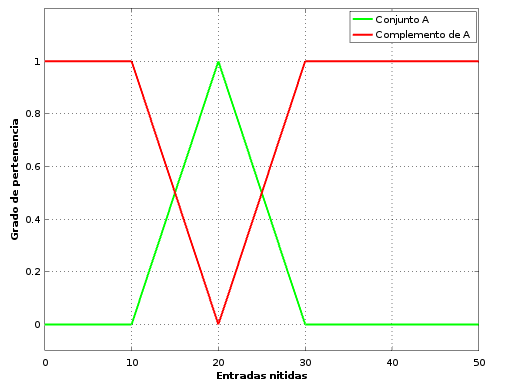
\includegraphics[width=8cm]{graficas/complemento.png}
\end{grafico}
\subsubseccion{Diferencia}
La diferencia estándar de $A$ y $B$ es el conjunto borroso $C$ en $X$, tal que su función de pertenencia $\mu_{C}(x):X \rightarrow [0, 1]$ está definida por medio de la proposición $\mu_{C}= \min \{\mu_{A}(x), 1 - \mu_{B}(x) \}$  para cada $x \in X$. Se denota $A-B$.
El \refgrafico{graficoDiferencia} muestra la diferencia estándar de dos conjuntos borrosos con funciones de pertenencia trapezoidales:
\begin{grafico}[titulo = Diferencia estandar en conjuntos difusos, etiqueta = graficoDiferencia]
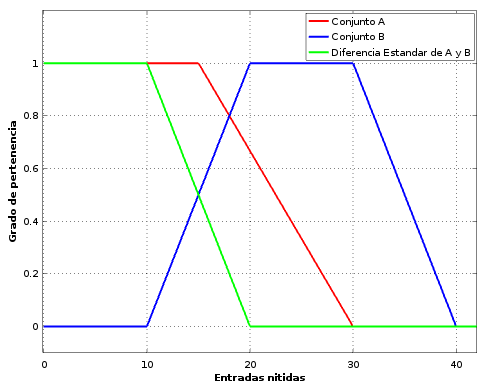
\includegraphics[width=8cm]{graficas/diferencia.png}
\end{grafico}
\\
Puesto que $\min \{\mu_{A}(x), 1 - \mu_{B}(x)\} = \min \{\mu_{A}(x), \mu_{\bar{B}}(x)\} =\mu_{A \cap \bar{B} }(x)$, entonces $(\forall x \in X)[\mu_{A - B }(x) = \mu_{A \cap \bar{B} }(x)]$.
\\
Luego, $A - B = A \cap \bar{B}$, es decir, la diferencia estándar de $A$ y $B$ es el conjunto difuso que se obtiene mediante la intersección estándar de $A$ y el complemento de $B$.
\subseccion{Lógica difusa y variables lingüísticas}
El término ``lógica difusa'' ha sido utilizado con dos significados diferentes. En un sentido conceptual, se refiere a un sistema lógico que generaliza la lógica clásica bivalente, para razonamiento bajo incertidumbre. En un sentido procedimental, la lógica difusa se refiere a los métodos y las técnicas que emplean conjuntos borrosos.\\
\\
La lógica difusa tiene una faceta relacional, que trata principalmente de la
representación y manipulación de funciones y relaciones definidas en forma
imprecisa. Esta faceta es fundamental en aplicaciones en áreas de información, control automático y modelado de sistemas. La lógica difusa es considerada como un campo de estudio dentro de la Inteligencia Artificial \cite[]{yen1999fuzzy}. La lógica difusa permite desarrollar sistemas y tecnologías computacionales con un manejo adecuado de incertidumbre en la información para realizar razonamientos y resolver problemas que requieran de inteligencia.\\
\\
\citet{trillas1992aplicaciones},  afirman que la lógica difusa permite representar el conocimiento común en un lenguaje matemático especial (el de la teoría de los subconjuntos borrosos y las distribuciones de posibilidad a ellos asociadas) y, a través de un cálculo lógico que flexibiliza la noción operativa de verdad, vista como predicado singular, permite efectuar inferencias aproximadas a partir de patrones de razonamiento que reproducen, aceptablemente, los métodos usuales de razonamiento que son, mayoritariamente, de tipo lingüístico cualitativo y no necesariamente cuantitativos. Por descontado, con posibilidad de reinterpretación de los resultados finales obtenidos a través de fórmulas, es un auxiliar común que presentan las matemáticas.\\
Una variable lingüística \cite[]{zadeh1975concept} es una $5-upla(x, T_{x}, U, G, M)$, en la cual:
\begin{viñetas}
\item $x$ es el nombre de la variable.
\item $T_{x}$ es el conjunto de términos lingüísticos referidos a la variable $x$.
\item $U$ es el universo del discurso en el contexto de la variable $x$.
\item $G$ es una regla sintáctica para generar los nombres de valores de $x$. 
\item $M: \rightarrow \F (U)$ es la regla semántica que asigna a cada término lingüístico $t \in T_{x}$ su significado. $M(t) \in \F (U)$, siendo $\F (U)$ la familia de conjuntos borrosos en $r$.
\end{viñetas}

\subseccion{Medidas de comparación entre conjuntos borrosos}
\\
\citet{zadeh1971similarity}, define la noción de similitud (similarity) como la generalización de la noción de equivalencia. Los conjuntos borrosos son utilizados en las mediciones de similitudes y disimilitudes entre objetos por su capacidad de representar información subjetiva resultante de la complejidad del mundo real. Las medidas de similitud entre conjuntos borrosos pueden tener una motivación de teoría de conjuntos o una motivación geométrica. Entonces, las medidas de similitud se pueden distinguir en dos clases: la basada en teoría de conjuntos y la geométrica.
A continuación, se hace una descripción de medidas de similitud entre conjuntos borrosos para cada una de estas clases.

\subseccion{Comparación de Objetos con Atributos Difusos}
La comparación y descripción de objetos es una operación habitual en muchos dominios: psicología, analogía, ciencias físicas, procesador de imágenes, agrupamiento (``clustering''), razonamiento deductivo, razonamientos basados en casos, entre otros campos. Estas comparaciones frecuentemente se basan en medidas que intentan determinar qué puntos tienen en común ambos objetos, es decir, medidas de similitud \cite[]{bouchon2008similarities}.\\
\\
La comparación de objetos con descripciones imperfectas, afectadas con imprecisiones e inexactitudes, puede ser tratada utilizando conjuntos borrosos para representar tales descripciones.

\subseccion{Toma de decisiones con múltiples atributos}
El proceso de toma de decisiones implica una serie de pasos: identificación de los problemas, construcción de preferencias, evaluación de las alternativas, y determinación de las mejores alternativas \cite[]{simon1977causal, kleindorfer1993decision}.\\
En general, tres tipos de análisis formal pueden emplearse para resolver problemas de toma de decisiones \cite[]{bell1988descriptive, kleindorfer1993decision}:
\\
\begin{viñetas}
\item El análisis descriptivo, que se ocupa de los problemas donde los decisores (``Decision Makers'', DM) ofrecen soluciones particulares.
\item El análisis prescriptivo, el cual considera que los métodos DM deben utilizarse para mejorar sus decisiones.
\item El análisis normativo se centra en los problemas que los DM idealmente deberían abordar.
\\
\end{viñetas}
La toma de decisiones es muy intuitiva al considerar los problemas de un criterio único, ya que sólo hay que elegir la alternativa con la calificación de preferencia más alta. Sin embargo, cuando el DM evalúa alternativas con múltiples criterios, aparecen muchos problemas, tales como los pesos de los criterios de preferencia, la dependencia, y los conflictos entre los criterios, parecen complicar los problemas y necesitan ser superadas por métodos más sofisticados.\\
\\
Con el fin de hacer frente a los problemas MCDM, el primer paso es averiguar cuántos atributos o criterios existen en el problema y la forma de entender los problemas (es decir, la identificación de los problemas). A continuación, se debe recolectar los datos o informaciones adecuadas en las que las preferencias de DM se pueden reflejar correctamente (es decir, la construcción de las preferencias). Continuando con la construcción de un conjunto de posibles alternativas o estrategias con el fin de garantizar que se alcance el objetivo (es decir, la evaluación de las alternativas). Finalmente se selecciona un método apropiado para ayudar a evaluar y posicionar las alternativas o estrategias (es decir, encontrar y determinar la mejor alternativa).\\
\\
A continuación se presentan algunos métodos para la evaluación de sistemas de información: 

\subsubseccion{Medidas globales de similitud}
Más de un atributo puede ser comparado entre dos casos. El algoritmo aplicado cuando hay más de un atributo relevante, debe ser considerado. En esta situación, se puede calcular la similitud promedio ponderada \cite[]{pal2004foundations}. Si SM denota una medida global de similitud, se tendrá la siguiente fórmula:
\begin{ecuacion}{ecuacionMedidaSimilitud}
	{S}_{M}=\cfrac {\sum _{i=1}^{ n }{ { w }_{ { M }_{ i } }}}{\sum _{ i=1 }^{ n }{ { w }_{ i }}}
\end{ecuacion}
Donde $S_{M_{i}}$ es la $i-ésima$ medida local de similitud, y $w_{i}$ es un factor de peso asociado con la $i-ésima$ medida local de similitud que es proporcional a la importancia relativa que se le asigne al atributo relacionado.

\subsubseccion{Proceso Analítico Jerárquico (AHP)}
Es una técnica estructurada para tratar con decisiones complejas. En lugar de prescribir la decisión “correcta”, el AHP ayuda a los decisores a encontrar la solución que mejor se ajusta a sus necesidades y a su comprensión del problema. \citet{bernoulli1783sammlung} propuso el concepto de función de utilidad para reflejar búsqueda humana, como la máxima satisfacción, \citet{neumann1947theory}  presentaron la teoría del juego y modelo de comportamiento económico, que amplió los estudios sobre los  problemas del  comportamiento económico humano para la Toma de Decisiones con Atributos Múltiples (MADM), una cantidad cada vez mayor de la literatura se ha dedicado a este campo. En términos generales, los procedimientos de MADM pueden resumirse en seis pasos a saber \cite[]{dubois1980systems}:
\begin{viñetas}
\item \textbf{Paso 1:} Definir la naturaleza del problema.
\item \textbf{Paso 2:} Construir un sistema jerárquico para su evaluación (gráfica). 
\item \textbf{Paso 3:} Seleccionar el modelo de evaluación apropiada.
\item \textbf{Paso 4:} Obtener los pesos relativos y puntuación de rendimiento de cada atributo con respecto a cada alternativa.
\item \textbf{Paso 5:} Determinar la mejor alternativa de acuerdo con los valores de utilidad, que son el valor agregado de los pesos relativos, y las puntuaciones de rendimiento correspondiente a las alternativas.
\\
\end{viñetas}
Cabe destacar que \citet{keeney1976decision} sugieren cinco principios que deben seguirse para la formulación de los criterios: 
(1) La integridad, (2) La operatividad, (3) de descomposición, (4) no redundancia, y (5) tamaño mínimo .
\subsubsection{Método de valores propios}
AHP fue propuesto por \citet{saaty1977scaling} para modelar los procesos de toma de decisiones subjetivas basadas en múltiples atributos en un sistema jerárquico. A partir de ese momento, se ha utilizado ampliamente en la planificación empresarial, la selección de portafolios, y el análisis de costo/beneficio por las agencias gubernamentales para fines de asignación de recursos. Cabe destacar que todos los problemas de decisión se consideran como una estructura jerárquica en el AHP. El primer nivel indica el objetivo para el problema de decisión específico. En el segundo nivel, el objetivo se descompone de varios criterios y los niveles más bajos puede seguir este principio a dividirse en otros subcriterios. Por lo tanto, la forma general de la AHP se puede representar como se muestra en el \refgrafico{graficoAHP}.
\begin{grafico}[titulo = Forma general de la AHP, etiqueta=graficoAHP]
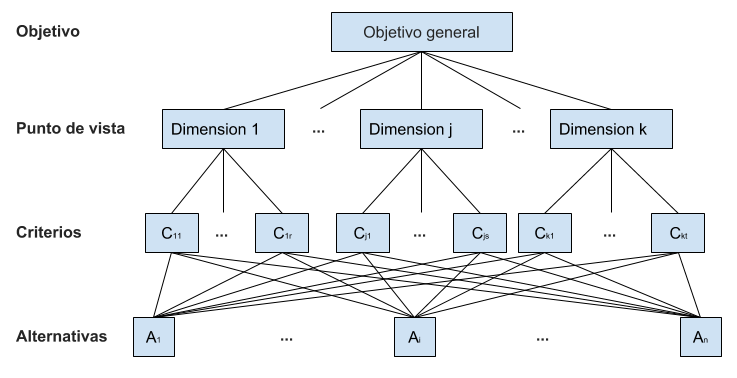
\includegraphics[width=15cm]{graficas/AHP.png}
\end{grafico}
\subsubseccion{Escala de proporción en el AHP}El \refcuadro{tablaEscalaAHP} representa la escala de índices que se emplea para comparar el peso entre los criterios de importancia de acuerdo con el significado lingüístico de 1 a 9 para denotar desde la misma importancia(1) a la extrema importancia(9).
\begin{cuadro}[titulo= Escala de proporción en el AHP, etiqueta = tablaEscalaAHP]{|p{1.8cm}|c|c|c|c|c|p{2cm}|}
\hline
Intensidad  & 1 & 3 & 5 & 7 & 9 & 2,4,6,8 \\
\hline
Termino lingüístico & Igual & Moderada & Fuerte & Demostrada & Extrema & Valores intermedios \\
\hline
\end{cuadro}
Además, con el fin de garantizar la coherencia de la percepción subjetiva y la exactitud de los pesos comparativos, se sugieren dos índices, el índice de consistencia (C.I.) y la relación de la consistencia (C. R.). La ecuación del C.I. se puede expresar como:
\begin{ecuacion}{ecuacionCI}
C.I.=\cfrac { (\mu _{ \max}-n)}{(n-1)}
\end{ecuacion}
Donde $\mu _{ \max}$ es el valor propio más grande, y $n$	 representa los números de los atributos. \citet{saaty1980analytic} sugirió que el valor del $C.I.$ no debe exceder de $0,1$ para un resultado de confianza. Por otro lado, la $C.R.$ se puede calcular como:
\begin{ecuacion}{ecuacionCR}
C.R.=\cfrac {C.I.}{R.I.}
\end{ecuacion}
El $R.I.$ para diferentes tamaños matriciales.
\begin{cuadro}[titulo= Escala de proporción en el AHP, etiqueta = tablaEscalaAHP]{|l|l|l|l|l|l|l|l|l|l|l|l|}
\hline
$N.E.$ & 3 & 4 & 5 & 6 & 7 & 8 & 9 & 10 & 11 & 12 & 13 \\
\hline
R.I. &  0.52 & 0.89 & 1.11 & 1.25 & 1.35 & 1.40 & 1.45 & 1.49 & 1.51 & 1.54 & 1.56
  \\
\hline
\end{cuadro}
El C. R. debe ser inferior a 0,1 para obtener un resultado fiable y 0,2 es el nivel máximo tolerado.\\
\\
En las aplicaciones a menudo es conveniente trabajar con números difusos triangulares debido a su simplicidad computacional y son útiles en la promoción de la representación y tratamiento de la información en un entorno difusa. 
\subsubseccion{Integración de AHP con los conjuntos difusos}
La metodología AHP Difusa considera la incorporación de números difusos, donde por conveniencia se utilizan números difusos triangulares (``Triangular Fuzzy Numbers'' ,TFN) debido a su simplicidad computacional. Inicialmente utiliza los números difusos para indicar el nivel de intensidad o importancia relativa que un factor de la jerarquía tiene por sobre otro. A partir de estas comparaciones se construye la matriz de comparaciones con números triangulares.
\begin{ecuacion}{ecuacionMatriz}
\tilde { A } = \begin{bmatrix} 1 & \tilde { { a } }_{ 12 }  & ... & \tilde { { a } }_{ 1n }  \\ \tilde { { a } }_{ 21 }  & 1 & ... & \tilde { { a }}_{ 2n }   \\ ... & ... & ... & ... \\ \tilde { { a } }_{ n1 }  & ... & ... & 1 \end{bmatrix}
\end{ecuacion}
Donde, $\tilde {{a}}_{ij}$ es un número triangular difuso, $\tilde {{a}}_{ij} = (l_{ij}, m_{ij}, n_(ij))$,   $\tilde {{a}}_{ji}=1/\tilde {{a}}_{ij}$. Para cada $TFN$, $\tilde {{a}}_{ij}$ o $M=(l, m, n)$, Es función de pertenencia de  $\tilde {{a}}_{ij}(x)$  o $M(x)$, siendo $-\infty \leq x \leq \infty$ para el intervalo cerrado $[0, 1]$.\\
\\
La mejor alternativa es obtenida consecuentemente a partir de un sistema de clasificación para números difusos.  El método AHP es un método que permite atribuir pesos donde valores numéricos no pueden ser obtenidos directamente. Este método trabaja a partir de una matriz donde se localizan las comparaciones entre pares, según la importancia o preponderancia relativa que un elemento de la jerarquía tenga sobre otro.


\subsubseccion{Técnica para el orden de preferencia por similitud con solución ideal (TOPSIS)}

El método TOPSIS es un modelo de decisión propuesto para ordenar preferencias por similitud con una solución ideal, es por tanto un método de clasificación (ranking). Fue desarrollado por \citet{hwang1981lecture} y mejorada por los autores \citet{chen1992fuzzy}, también trabajaron \citet{zeleny1994search}, \citet{lai1994topsis}, \citet{garcia2012rank} entre otros. TOPSIS es un método de decisión multicriterio de ordenación para identificar las soluciones de un conjunto finito de alternativas. El principio básico es que la alternativa elegida debe tener la menor distancia a la solución ideal positiva y la mayor distancia a la solución ideal negativa. Una solución ideal se define como una colección de puntuaciones o valores en todos los atributos considerados en la decisión, pudiendo suceder que tal solución sea inalcanzable. El vector compuesto por los mejores valores del j-ésimo atributo respecto de todas las alternativas posibles es quien recibe el nombre de ``solución ideal positiva'' (SIP); recíprocamente, la ``solución ideal negativa'' (SIN) será aquella cuyo vector contenga los peores valores en todos los atributos. A fin de definir la solución ideal, el método  TOPSIS establece un índice de similaridad que se construye combinando la proximidad al ideal positivo y la lejanía respecto al ideal negativo. El procedimiento de TOPSIS puede expresarse en una serie de pasos que pueden verse en \citet{jahanshahloo2006algorithmic}, y se describen a continuación.\\
Calcular la matriz de decisión normalizado. El valor de $n_{ji}$ normalizado se calcula como
\begin{ecuacion}{ecuacionNormalizacion}
n_{ ij }=\cfrac { x_{ ij } }{ \sqrt { \sum _{ i=1 }^{ n }{ { x }_{ ij }^{ 2 }\quad ,\quad i = 1,\quad 2,\quad ...,\quad m;\quad j = 1,\quad 2,\quad ...,n }  }  } 
\end{ecuacion}
Luego, calcular la matriz de decisión de pesos normalizados. Los pesos normalizados $v_{ij}$ son calculados como
$v_{ij}=w_{ij}n_{ij}; i=1, 2,..., m; j=1,2,..., n$
donde  $w_{j}$ es el peso del $i-ésimo$ atributo o criterio, y
\begin{ecuacion}{ecuacionPesoICriterio}
\sum _{ j=1 }^{ n }{ w_{ i } } =1
\end{ecuacion}

Determinar la solución ideal positiva y la solución ideal negativa:
\begin{ecuaciones}
{ A }^{ + }=\{ { v }_{ 1 }^{ + },\quad { v }_{ 2 }^{ + },\quad ...,\quad { v }_{ n }^{ + }\} =\left\{ ({ max }_{ j }v_{ ij }|i\in I),\quad ({ min }_{ j }v_{ ij }|i\in J) \right\} \\
{ A }^{ - }=\{ { v }_{ 1 }^{ - },\quad { v }_{ 2 }^{ - },\quad ...,\quad { v }_{ n }^{ - }\} =\left\{ ({ min }_{ j }v_{ ij }|i\in I),\quad ({ max }_{ j }v_{ ij }|i\in J) \right\}
\end{ecuaciones}
Calcular las medidas de separación, usando la distancia Euclidiana $n-dimensional$. La separación de cada alternativa de la solución ideal, es dada como:\\
\begin{ecuacion}{ecuacionpositiva}
{ d }_{ i }^{ + }={ \left\{ \sum _{ j=1 }^{ n }{ { ({ v }_{ ij }-{ v }_{ i }^{ + }) }^{ 2 } }  \right\}  }^{ \sfrac { 1 }{ 2 }  };\quad i=1,2,\quad ...,m
\end{ecuacion}
Del mismo modo, la separación de la solución ideal negativa se da como:
\begin{ecuacion}{ecuacionpositiva}
{ d }_{ i }^{ - }={ \left\{ \sum _{ j=1 }^{ n }{ { ({ v }_{ ij }-{ v }_{ i }^{ - }) }^{ 2 } }  \right\}  }^{ \sfrac { 1 }{ 2 }  };\quad i=1,2,\quad ...,m
\end{ecuacion}
Calcular la cercanía relativa a la solución ideal. La proximidad relativa de la alternativa  $A_{i}$ con respecto a $A^{+}$ se define como
\begin{ecuacion}{ecuacioncercaniarelat}
{ R }_{ i }={ { d }_{ i }^{ - } }/{ ({ d }_{ i }^{ + }-{ d }_{ i }^{ - }),\quad i=1,2,\quad ...,\quad m }
\end{ecuacion}
Desde $d_{i} \geq 0$  y  $d_{i} \geq 0$ , entonces claramente, $R_{i}\in [0,1]$.\\
\\
La clasificar las alternativas utilizando este índice, permite ordenar las alternativas respecto a las preferencias en forma descendiente, el principio básico del método TOPSIS es que la alternativa elegida debe tener la ``distancia más corta'' de la solución ideal positiva y el ``distancia más lejana'' de la solución ideal negativa.
\subseccion{Aplicaciones móviles y sus características}
\citet{santiago2015mobile} definen a las aplicaciones móviles como aplicaciones informáticas diseñadas para ser ejecutada en teléfonos inteligentes, tabletas y otros dispositivos móviles y que permite a los usuarios efectuar una tarea concreta de cualquier tipo ---profesional, de ocio, educativas, de acceso a servicios, entre otras---, facilitando las gestiones o actividades a desarrollar.
A nivel de programación, existen varias formas de desarrollar aplicaciones. Cada una de ellas tiene diferentes características y limitaciones, especialmente desde el punto de vista técnico.
\citet{cuello2013disenando} definen tres tipos de aplicaciones; las nativas, las web y las híbridas. A continuación se describe cada una de estas:  

\subsubseccion{Aplicaciones nativas}

Las aplicaciones nativas son aquellas que han sido desarrolladas con el software que ofrece cada sistema operativo a los programadores, llamado genéricamente Software Development Kit o SDK. Así, Android, iOS y Windows Phone tienen uno diferente y las aplicaciones nativas se diseñan y programan específicamente para cada plataforma, en el lenguaje utilizado por el SDK.\\
Este tipo de apps se descarga e instala desde las tiendas de aplicaciones ---con ciertas excepciones en el caso de Android, que veremos en el capítulo «Lanzando la app»--- sacando buen partido de las diferentes herramientas de promoción y marketing de cada una de ellas.\\
Las aplicaciones nativas se actualizan frecuentemente y en esos casos, el usuario debe volver a descargarlas para obtener la última versión, que a veces corrige errores o añade mejoras.
Una característica generalmente menospreciada de las apps nativas, es que pueden hacer uso de las notificaciones del sistema operativo para mostrar avisos importantes al usuario, aun cuando no se esté usando la aplicación, como, por ejemplo, los mensajes de Whatsapp.\\
Además, no requieren de Internet para funcionar, por lo que ofrecen una experiencia de uso más fluida y están realmente integradas al teléfono, lo cual les permite utilizar todas las características de hardware del terminal, como la cámara y los sensores (GPS, acelerómetro, giróscopo, entre otros).\\
A nivel de diseño, esta clase de aplicaciones tiene una interfaz basada en las guías de cada sistema operativo, logrando mayor coherencia y consistencia con el resto de aplicaciones y con el propio SO. Esto favorece la usabilidad y beneficia directamente al usuario que encuentra interfaces familiares.\\

\subsubseccion{Aplicaciones web}

La base de programación de las aplicaciones web -también llamadas webapps- es el HTML, conjuntamente con JavaScript y CSS, herramientas ya conocidas para los programadores web.
En este caso no se emplea un SDK, lo cual permite programar de forma independiente al sistema operativo en el cual se usará la aplicación. Por eso, estas aplicaciones pueden ser fácilmente utilizadas en diferentes plataformas sin mayores inconvenientes y sin necesidad de desarrollar un código diferente para cada caso particular.
Las aplicaciones web no necesitan instalarse, ya que se visualizan usando el navegador del teléfono como un sitio web normal. Por esta misma razón, no se distribuyen en una tienda de aplicaciones, sino que se comercializan y promocionan de forma independiente.\\
Al tratarse de aplicaciones que funcionan sobre la web, no es necesario que el usuario reciba actualizaciones, ya que siempre va a estar viendo la última versión. Pero, a diferencia de las apps nativas, requieren de una conexión a Internet para funcionar correctamente.\\
Adicionalmente, tienen algunas restricciones e inconvenientes en factores importantes como gestión de memoria y no permiten aprovechar al máximo la potencia de los diferentes componentes de hardware del teléfono.
Las aplicaciones web suelen tener una interfaz más genérica e independiente de la apariencia del sistema operativo, por lo que la experiencia de identificación del usuario con los elementos de navegación e interacción, suele ser menor que en el caso de las nativas.

\subsubseccion{Aplicaciones hibridas}
Este tipo de aplicaciones es una especie de combinación entre las dos anteriores. La forma de desarrollarlas es parecida a la de una aplicación web ---usando HTML, CSS y JavaScript---, y una vez que la aplicación está terminada, se compila o empaqueta de forma tal, que el resultado final es como si se tratara de una aplicación nativa.
Esto permite casi con un mismo código obtener diferentes aplicaciones, por ejemplo, para Android y iOS, y distribuirlas en cada una de sus tiendas.
A diferencia de las aplicaciones web, éstas permiten acceder, usando librerías, a las capacidades del teléfono, tal como lo haría una app nativa.2
Las aplicaciones híbridas, también tienen un diseño visual que no se identifica en gran medida con el del sistema operativo. Sin embargo, hay formas de usar controles y botones nativos de cada plataforma para apegarse más a la estética propia de cada una.
Existen algunas herramientas para desarrollar este tipo de aplicaciones. Apache Cordova3 es una de las más populares, pero hay otras, como Icenium4, que tienen la misma finalidad.
\subsubseccion{Desarrollo de aplicaciones móviles}
De acuerdo con \citet{wasserman2010software} en muchos aspectos, el desarrollo de aplicaciones móviles es similar a la ingeniería de software para otros tipos de aplicaciones. Problemas comunes incluyen la integración con el hardware del dispositivo, así como los problemas tradicionales de la seguridad, el rendimiento, la fiabilidad y las limitaciones de almacenamiento. Sin embargo, las aplicaciones móviles presentan algunos requisitos adicionales que se encuentran menos comúnmente en aplicaciones de software tradicionales, incluyendo:
\begin{enumeracion}
\item Posible interacción con otras aplicaciones - los dispositivos más integrados sólo tienen software instalado de fábrica, pero los dispositivos móviles pueden tener numerosas aplicaciones de diversas fuentes, con la posibilidad de interacciones entre ellos.
\item La manipulación del sensor - los dispositivos móviles más modernos, por ejemplo, ``teléfonos inteligentes'', incluyen un acelerómetro que responde al movimiento del dispositivo, una pantalla táctil que responde a numerosos gestos, junto con los bienes y / o teclados virtuales, un sistema de posicionamiento global, un micrófono utilizable por aplicaciones distintas de las llamadas de voz, una o más cámaras, y protocolos de red múltiples.
\item Aplicaciones nativas e híbridas (web móvil) - dispositivos más integrados utilizan sólo las instaladas directamente en el dispositivo de software, pero los dispositivos móviles a menudo incluyen aplicaciones que invocan servicios a través de la red telefónica o Internet a través de un navegador web y afectan a los datos en el dispositivo.
\item Familias de plataformas de hardware y software - la mayoría de dispositivos embebidos ejecutan código que está hecho a la medida para las propiedades de ese dispositivo, pero los dispositivos móviles pueden tener que soportar las aplicaciones que se han escrito para todos los variados dispositivos que soportan el sistema operativo, y también para diferentes versiones del sistema operativo. Un desarrollador de Android, por ejemplo, debe decidir si se ha de construir una aplicación única o múltiples versiones para correr en la amplia gama de dispositivos Android y versiones del sistema operativo.
\item Seguridad - los dispositivos más integrados son ``cerrados'', en el sentido de que no hay manera fácil de atacar el software embebido y afectar a su funcionamiento, pero las plataformas móviles están abiertas, permitiendo la instalación de nuevas aplicaciones, y un ``malware'' puede afectar el funcionamiento global del dispositivo, incluida la transmisión encubierta de datos locales por una aplicación de este tipo.
\item Las interfaces de usuario - con una aplicación embebida hecha a la medida, el desarrollador puede controlar todos los aspectos de la experiencia del usuario, pero en una aplicación móvil deben compartir elementos comunes de la interfaz de usuario con otras aplicaciones y deben adherirse a lo desarrollado externamente para las directrices de la interfaz de usuario, muchas de las cuales se implementan en los kits de desarrollo de software (``Software development kit'', SDK) que forman parte de la plataforma.
\item Complejidad de las pruebas - mientras que las aplicaciones nativas se pueden probar de forma tradicional o a través de un emulador basado en PC, las aplicaciones web móviles son particularmente difíciles de probar. No sólo tienen muchos de los mismos problemas que se encuentran en aplicaciones de pruebas web; que además tienen problemas asociados con la transmisión a través de pasarelas y la red telefónica.
\item Consumo de energía - muchos aspectos de una aplicación afecta el consumo de energía del dispositivo y por lo tanto la duración de la batería. Dispositivos dedicados pueden ser optimizados para una máxima duración de la batería, pero las aplicaciones móviles pueden inadvertidamente hacer un uso extensivo de los recursos del consumo de batería.


\end{enumeracion}

%Si se va a usar el glosario
%\hacerglosario
